\documentclass[12pt]{article}
\usepackage{fancyhdr}     % Enhanced control over headers and footers 
\usepackage[T1]{fontenc}  % Font encoding
\usepackage{mathptmx}     % Choose Times font 
\usepackage{microtype}    % Improves line breaks      
\usepackage{setspace}     % Makes the document look like horse manure 
\usepackage{hyperref}
\hypersetup{
	colorlinks   = true, %Colours links instead of ugly boxes
	urlcolor     = blue, %Colour for external hyperlinks
	linkcolor    = black, %Colour of internal links
	citecolor   = black %Colour of citations
}
\usepackage{graphicx}
\usepackage{amsmath}
\usepackage{subcaption}
\usepackage{endnotes}
\usepackage{float}
\usepackage{algorithm}
\usepackage{algpseudocode}
\usepackage{multicol}
\usepackage{tikz}
\usetikzlibrary{snakes}
\usepackage{rotating}
\usetikzlibrary{positioning,shapes.multipart}
 \usepackage{listings}

\usepackage[style=apa,backend=biber,citestyle=numeric]{biblatex}
\addbibresource{../refs.bib}

\title{Bayesian Neural Networks}
\author{
	Blair, Taylor
	\and
	Sorgman, Ava
	\and
	Bekaert, Conor
}
\date{\today}
\let\footnote=\endnote

\usepackage{verbatim}

\pagestyle{fancy} % Default page style 
\lhead{Blair, Sorgman, Bekaert}
\chead{}
\rhead{\thepage}
\cfoot{}
\rfoot{}
\renewcommand{\headrulewidth}{1pt}
\renewcommand{\footrulewidth}{1pt}
\renewcommand{\theendnote}{\Roman{endnote}} 



\begin{document}
\doublespacing
\maketitle



%\begin{abstract}
%	Bayesian Neural Networks are...
%\end{abstract}

\tableofcontents

	
\section{Machine Learning}
	
% To understand the concept of deep learning, we first need to understand the broader area it is considered a subset of; machine learning. 
%Machine learning is considered to be a branch of artificial intelligence (AI) with the goal to help AI “learn” more, but specifically in a way that imitates the human process of learning through the use of data and algorithms\cite{ibmWhatIsML}. 
Machine learning includes a variety of topics of which artifical intelligence (AI) and neural networks are a subset. Neural networks in particular involve an abstract imitation of the human brain using simulated neurons which is trained on data using particular algorithms. 

The term supervised learning refers to a specific common method of machine learning that uses a labeled dataset to train a model to correctly predict the labels via some training algorithm. A classification problem in supervised learning involves predictions where all labels are grouped into a set of categories. The training process can be broken down into three major steps, which include a decision process, an error function, and an optimization process \cite{berkelyWhatIsML}. The decision process is the set of steps the algorithm takes after receiving the data based on the goal of the model. The second step in the process is the error function, which is the method of measuring chosen to see if the algorithm gave a ``good" or ``bad" input. The two most common choices of the error function are a simple yes or no on whether a data point was classified correctly in the case of classification, or the difference in value between the predicted outcome and the actual observed outcome for continuous values. Finally, the third and last step is the part of the process that implements learning. This step, the updating or optimization process, requires the algorithm to review the past data and outputs of the error function in order to better correct its decision-making process in the future.

Throughout this report, we will often use the terms machine learning, deep learning, and neural networks. It is important to note that although these are fundamentally related fields, deep learning is a subfield of neural networks that in particular focuses on more complicated neural networks, while neural networks are a subfield in machine learning. 

We will be training a classifier on labeled images in a supervised learning process to predict what is depicted in the image from a range of possibilities such as dog, cat, and plane. These images come from the CIFAR-10 dataset, which will be discussed more in detail later in this paper.


% EDIT THIS SECTION But, back to deep learning! What sets deep learning apart from the more general machine learning is that unlike the supervised learning process that was described before, deep learning does not necessarily have to use pre labelled data sets. It can, if required, but the point of a deep learning algorithm is that one feature of the algorithm is that it itself can distinguish between the different types of data purely by looking at the data. This process of built in categorical distinction is extremely helpful, as it limits human interaction and interventions that are required in the learning process, as large amounts of data do not need to be “processed by hand” in order for the algorithm to make use of them (2). Deep learning models work through a “layering” process, where multiple layers of the original three steps listed above work together in the algorithmic process.

	
\subsection{Introduction to Neural Networks}


\begin{figure}[H]
	\centering
	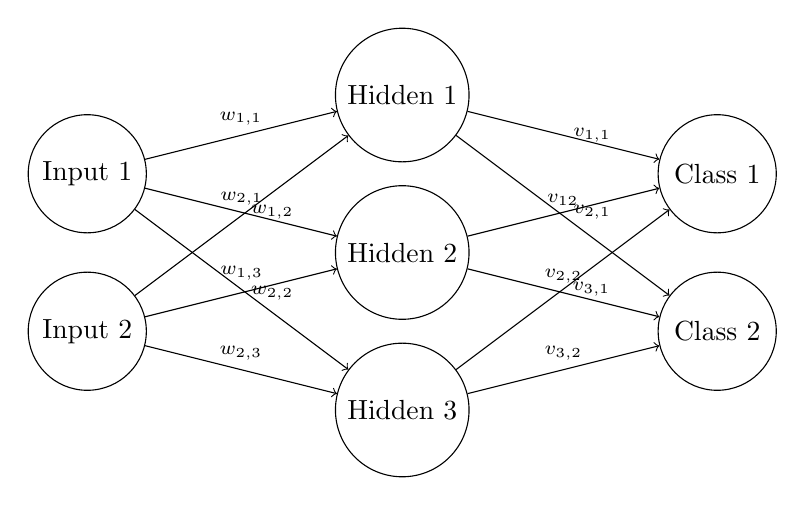
\begin{tikzpicture}
		% Define node styles
		\tikzstyle{neuron} = [circle, draw, minimum size=1.5cm];
		\tikzstyle{weight} = [font=\scriptsize];
		
		% Input layer (2 neurons)
		\node[neuron] (input1) at (-2,1) {Input 1};
		\node[neuron] (input2) at (-2,-1) {Input 2};
		
		% Hidden layer (3 neurons)
		\node[neuron] (hidden1) at (2,2) {Hidden 1};
		\node[neuron] (hidden2) at (2,0) {Hidden 2};
		\node[neuron] (hidden3) at (2,-2) {Hidden 3};
		
		% Output layer (2 neurons for classification)
		\node[neuron] (output1) at (6,1) {Class 1};
		\node[neuron] (output2) at (6,-1) {Class 2};
		
		% Connections with weights
		\draw[->] (input1) -- node[weight, above] {$w_{1,1}$} (hidden1);
		\draw[->] (input2) -- node[weight, above] {$w_{2,1}$} (hidden1);
		\draw[->] (input1) -- node[weight, right] {$w_{1,2}$} (hidden2);
		\draw[->] (input2) -- node[weight, right] {$w_{2,2}$} (hidden2);
		\draw[->] (input1) -- node[weight, above] {$w_{1,3}$} (hidden3);
		\draw[->] (input2) -- node[weight, above] {$w_{2,3}$} (hidden3);
		\draw[->] (hidden1) -- node[weight, right] {$v_{1,1}$} (output1);
		\draw[->] (hidden2) -- node[weight, right] {$v_{2,1}$} (output1);
		\draw[->] (hidden3) -- node[weight, right] {$v_{3,1}$} (output1);
		\draw[->] (hidden1) -- node[weight, above] {$v_{12}$} (output2);
		\draw[->] (hidden2) -- node[weight, above] {$v_{2,2}$} (output2);
		\draw[->] (hidden3) -- node[weight, above] {$v_{3,2}$} (output2);
	\end{tikzpicture}
	\caption{Example neural network}
	\label{fig:example-nn}
\end{figure}

There are many effective introductions to neural networks to any level of detail available elsewhere, but we will present a summary of the core concepts here. 

Many models for analyzing data involve making an assumption about the functional form of the outputs given the inputs or predictors. Neural networks are no exception - at the most basic conceptual level, a neural network is just a really complicated function that has the potential to represent many patterns through its complexity. Their name comes from the inspiration they take from the human brain, the idea that enough neurons with enough connections between them can encode everything needed for effective predictions. Indeed, the fundamental unit of a neural network is a neuron and its associated connections.

Neural networks are typically organized in a series of layers of many neurons, where each individual neuron of one layer is connected to every neuron of the previous layer. Data flows from an initial input layer, through hidden layers, then into the outputs as visualized in Figure \cite{fig:example-nn}. The connections are assigned certain weights, which measure the influence of a neuron on the next layer. The next section will describe the structure of neurons in a linear layer, which is a typical type of layer. %This structure ultimately yields a complicated yet well-defined function because every step is a clearly-defined arithmetic operation, and they are all composed into a single whole. %Neural networks can have different architectures depending on the organization and types of layers involved.


\subsection{Neural Network Neurons}

% As shown in Figure \ref{fig:neuron}, any single neuron is connected to the neurons $x_1, x_2, ..., x_n$ from the previous layer. The outputs of the previous neurons become the inputs to the new neuron by means of connections with weights $w_1, w_2, ..., w_n$ associated with them (each previous neuron has a certain weight). The neuron itself first takes a value calculated as a weighted sum $\sum_i w_i x_i$ of the inputs $x_i$ to it, then typically an additive bias is included. Lastly, the value is passed through an activation function which restricts the value to a certain range, typically $[0,1]$. 

%The weights and the biases of a neural network are the parameters, and they are the values that are tuned in the training process. In a sense, they represent the "memory" of the network, whatever it has learned from training. For any particular network architecture (meaning the choice of types of layers and their order), once the model has been trained with a particular architecture, the parameters are all you need to run that network on new data to make predictions. 


\begin{figure}[H]
	\centering
	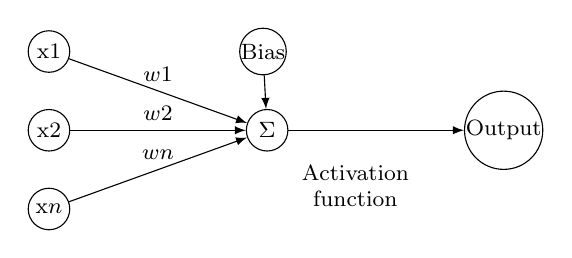
\begin{tikzpicture}[
		neuron/.style={
			circle,
			draw,
			minimum size=1.5em,
			inner sep=0pt,
		},
		font=\footnotesize,
		>=latex
		]
		% Draw the neuron
		\node [neuron] (neuron) at (0,0) {$\Sigma$};
		% Draw the input nodes and labels
		\foreach \i/\txt in {1/$1$,2/$2$,3/$n$} {
			\node [neuron,left=of neuron] (input\i) at (-1.5,-\i +2) {x\txt};
			\draw[->] (input\i) -- node[above] {$w$\txt} (neuron);
		}
		% Draw the bias node and label
		\node [neuron,left=of neuron] (bias) at (1.25,1) {Bias};
		\draw[->] (bias) -- node[right] {} (neuron);
		% Draw the activation function label
		\node[align=center,below right =0.5em of neuron] {Activation \\ function};
		% Draw the output node and label
		\node [neuron,right=of neuron] (output) at (1.5,0) {Output};
		\draw[->] (neuron) -- node[above] {} (output);
		% Draw the relevant functions
		%\draw[->] (0,-1.5) -- (0,-2.5) node[midway,right] {Weighted sum};
		%\draw[->] (-1.5,-3.5) -- (-1.5,-4.5) node[midway,left] {Bias};
		%\draw[->] (1.5,-0.5) -- (1.5,-1.5) node[midway,right] {Activation};
		
		% Draw the activation function shape
		%\node[draw,rectangle,minimum width=2em,minimum height=2em] (actfunc) at (0,1) {};
		%\node[above=0.1em of actfunc] {ReLU};
		
	\end{tikzpicture}
	\caption{Neural network neuron}
	\label{fig:neuron}
\end{figure}

A neural network neuron in a linear layer is, in practice, a varying real scalar value. The value is produced from the values $X = (x_1, ..., x_n)$ of the neurons in the previous layer by taking the dot product of $X$ with the weight parameters $W = (w_1, ..., w_n)$, plus an additive bias $b$. This weighted sum $X \cdot W + b$ is then passed through some activation function $\text{Act}(\cdot)$ which applies a nonlinear transformation to improve efficiency. As such, the action of a particular layer on the previous layer's neurons to produce the next value can be characterized as $X_{i+1} = \text{Act}(X_{i} \cdot W_{i} + b_{i})$. Typical activation functions include the Rectified Linear Unit (ReLU) defined by $\text{ReLU}(x) = \max (0, x)$ and the sigmoid, $\sigma(x) = \frac{1}{1 + e^{-x}}$.

This process can be generalized to an entire layer at once via matrix multiplication (which encodes the dot product), and this also improves efficiency. These layers are nested interatively to the depth of the network - for example, a network with three linear layers could take the form
$$
	\text{ReLU}(\text{ReLU}(\text{ReLU}(x \times W_1 + b_1) \times W_2 + b_2) \times W_3 + b_3).
$$
A network architecture is generally defined by the depth (number of layers), the number of neurons/parameters in the layers, and the type of layer used. 


	
\subsection{Neural Network Training}
\label{subsection:neural-network-training}

To train a neural network requires a loss function $L$, such as the MSE or the cross-entropy loss (cross-entropy loss is essentially the log-likelihood loss from frequentist maximum likelihood estimation). An optimization process, typically a variant of stochastic gradient descent, adjusts the neural network parameters $\beta$ (the weights $W$ and biases $b$) to minimize this loss on the provided data. Stochastic gradient descent updates the parameters at each step by the formula
$$
\beta_{n+1} = \beta_n - \alpha (\nabla \ell(x_s, y_s, \beta)),
$$
where $\alpha$ is the \textit{learning rate}, which controls how quickly parameter adjustments are made. Minimization is implemented using a stochastic approximation of the gradient of the loss (hence the name stochastic gradient descent). The true loss $L(\beta)$ on the whole dataset $x, y$ is approximated via an averaged estimate $\ell(x_s, y_s, \beta)$ on a subset $(x_s, y_s)$ of the data. Gradients are calculated via \textit{backpropagation}, which is beyond the scope of this discussion, but essentially consists of iterated application of the chain rule. 

Each step of training is called an \textit{epoch}. In each epoch, the data passes through the network, the gradients are approximated via backpropagation, and the parameters are updated with this approximation. These parameters, matrices of weights and biases, \textit{are} the network once it is trained - they represent the "memory" of the network, whatever it has learned from the training data. Predictions are obtained as the outputs after passing new data through the same network architecture with these weights and biases specified. This is a "black box" model because there is no clear interpretation of the giant matrices of parameters - in the end, they're just floating-point numbers. 



\subsection{Convolutional Neural Networks }

\begin{figure}[H]
	\centering
	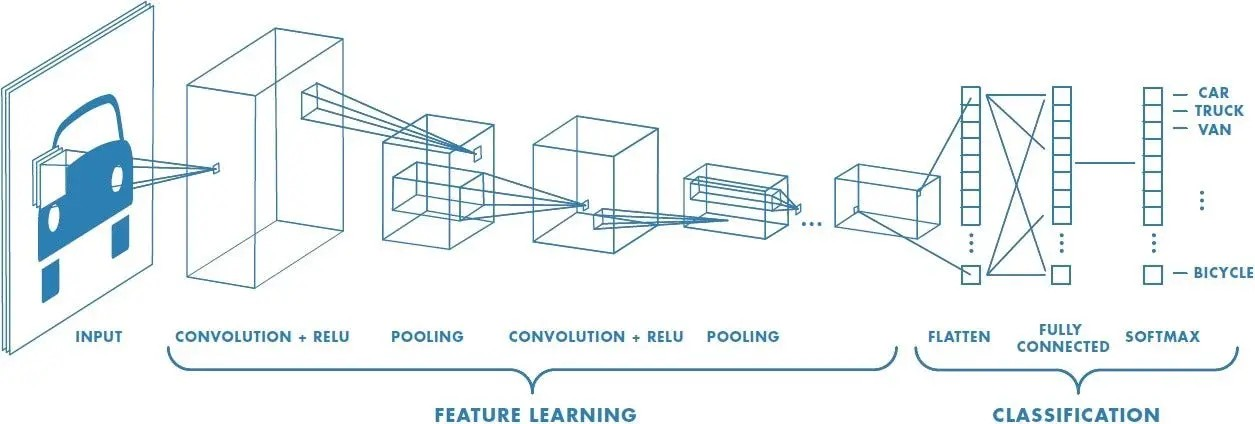
\includegraphics[width=.8\textwidth]{../Images/big-pic-cnn.jpg}
	\caption{CNN pipeline \cite{eli5CNN}}
	\label{fig:cnn-pipeline}
\end{figure}

Convolutional neural networks (CNN) are a type of neural network that is better suited for image recognition. While this might sound like a separate model structure, CNNs are largely the same. The primary difference from a traditional neural network is the convolutional layer, as highlighted in Figure \cite{fig:cnn-pipeline}. Instead of reading the entire image at once, a convolutional layer slides a small window over the image, shrinking that window even further by the application of a convolution operation. Once the window has slid over the entire image, a downsized image is formed that may encode useful information more densely. Because of this downsizing action, CNNs typically require fewer parameters relative to the traditional neural networks described previously, which improves training costs and the capabilities of the model. 

%IMAGE OF SLIDING (gif split)



\section{Bayesian Neural Networks}

\begin{figure}[H]
	\centering
	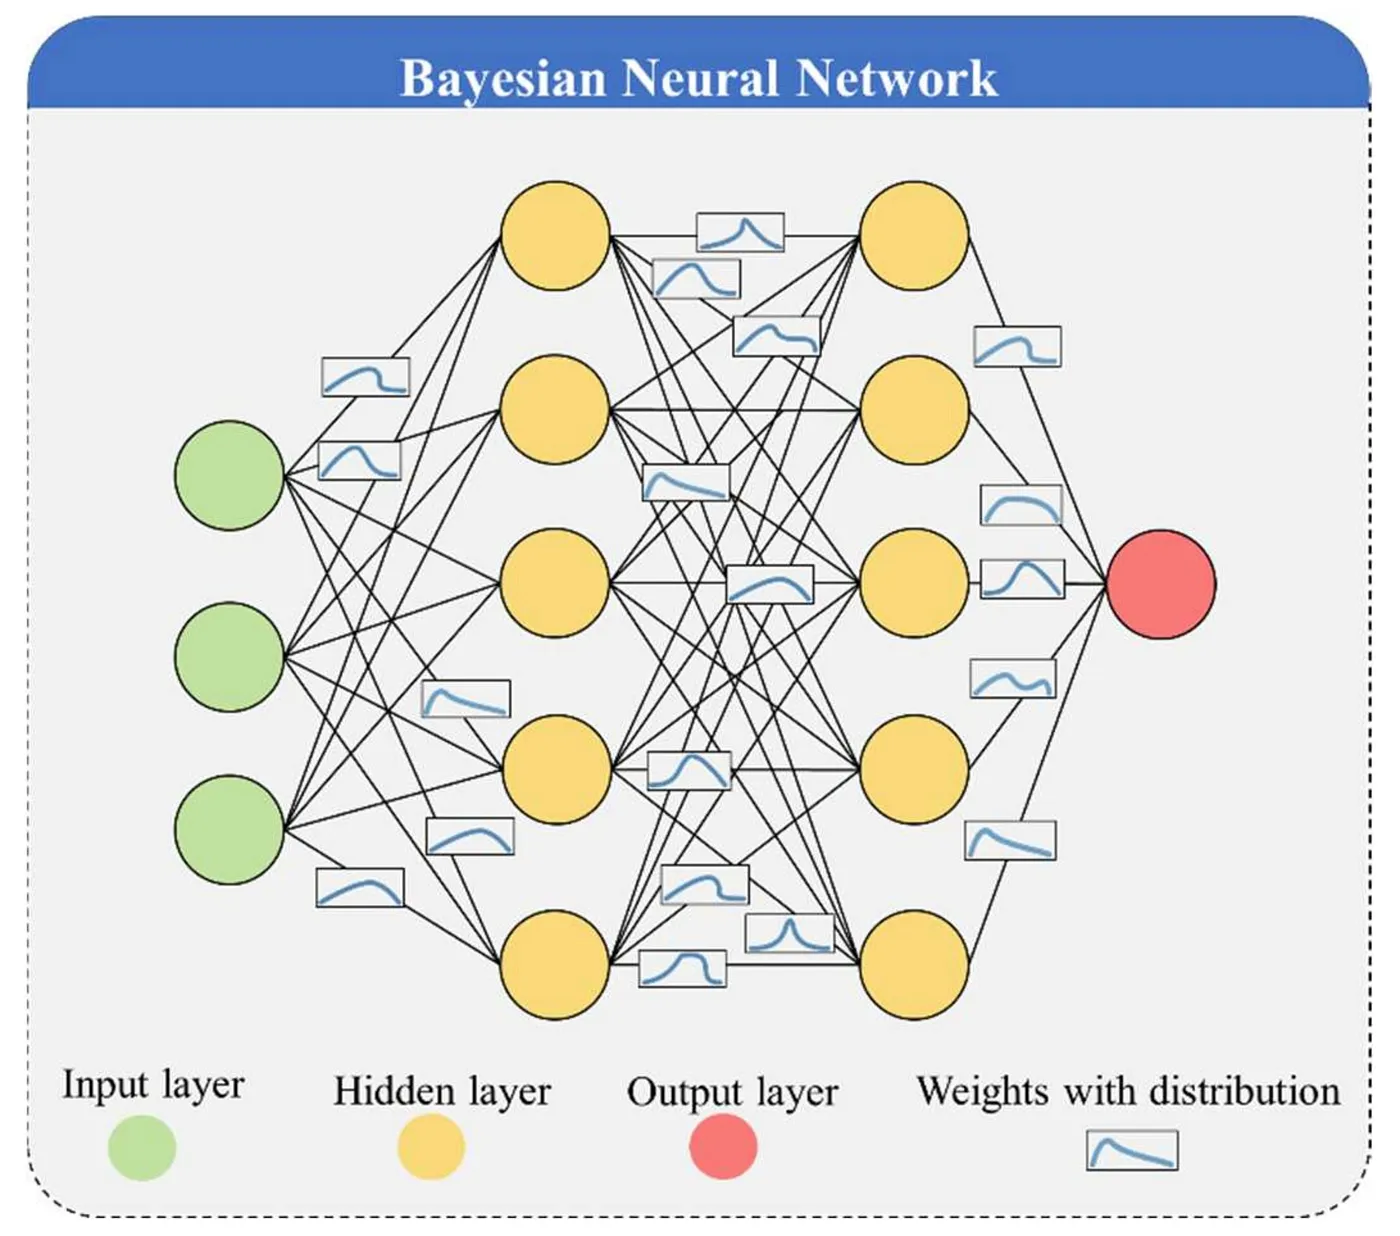
\includegraphics[width=.55\textwidth]{../Images/example_bnn.png}
	\caption{Example BNN  \cite{FleszarBNN}}
\end{figure}

Bayesian neural networks (BNN) are similar in principle to typical neural networks, but represent uncertainty in the predictions of a neural network by assigning probability distributions to the parameter (weight and bias) values and updating these distributions. This follows Bayesian principles, where rather than producing a single estimated value as in typical neural networks, the "evidence" provided by the data updates a distribution of possible true values. 

% take the same principle as your typical neural network, but factor in a measure of uncertainty into the prediction of the network. This uncertainty, of course, comes from the Bayesian theory of statistics, which believes that all events have some level of randomness, and thus must have uncertainty in their prediction. 

Uncertainty can be built into these models through prior probability distributions. 
%Uncertainty estimates of the model can be obtained from the parameters of the BNN in their probability distributions \cite{shridhar2019comprehensive}. 
The average estimate of the parameters is computed through multiple different models during the training process, which can regularize the network. However, it can be very difficult to calculate the model posterior of a BNN. Approximations of the posterior of the model are most often used, but those are often still very computationally intensive. Different methods of approximating the model's posterior is a current research topic within the field.

The two main types of uncertainty within a BNN are aleatoric uncertainty and epistemic uncertainty. Aleatoric uncertainty is a measure of the uncertainty in the observations, which is uncertainty that is inherent in any form of data. This type of uncertainty is modeled by placing a prior distribution over the output of the BNN model. In contrast, epistemic uncertainty is a measure of the uncertainty caused by the model and its predictions. It is modeled by a prior distribution over the model's weights, and an analysis of how much the weights of the model change when the data given to the model changes \cite{shridhar2019comprehensive}.

But what is so great about calculating uncertainty in our model? %Well, it's that our predictions become more uncertain. 
One of the major issues with neural networks as they are is they are highly prone to overfitting the data. Although they are great at predictions on the training data they are given, they often struggle with predictions on the testing data they are given due to the issue of overfitting. Many methods have been developed in order to regularize neural networks to work to prevent this from occurring, such as weight control measures. The Bayesian framework, and particularly the choice of prior distributions, builds this into the model, which helps prevent overfitting. 
%Using the Bayesian framework of uncertainty and building it into a model serves as a built-in prevention of overfitting.

%A Bayesian neural network introduces priors on the parameters $\theta$ of a neural network and uses the data to adjust these priors to reach posterior distributions for these parameters. 
Recall that a (trained) neural network is really just determined by its parameters - the weights and biases. This gives rise to the conceptual interpretation that a Bayesian neural network is an infinite ensemble of possible neural networks which can be sampled to obtain any number of individual networks. 
%(... could talk about how this enables comparison between networks, uncertainty, etc)

Constructing a Bayesian neural network involves selecting a model architecture and choosing the priors, which are also known as the "stochastic model" in this context. The definition of Bayesian neural networks provides flexibility, since the primary difference is that neuron weights get distributions instead of individual values. As a result, most model architectures that work for a typical neural network also work for a Bayesian version of that network. %Lastly, the training of a Bayesian neural network uses techniques such as MCMC for inference. 

% TODO: Fill in information about how distributions are imposed on a BNN. See other TODO with some progress at the end of the following subsection(s)
 


\subsection{Bayesian Neural Network Neuron}

A visualization of a Bayesian neuron appears in Figure \ref{fig:bnn-neuron}. It is in fact quite similar to Figure \ref{fig:neuron}, with the essential difference that the individual values from before have been replaced with distributions. Within a neuron, the distributions from input neurons are weighted by the weight distributions and combined together along with the bias distribution. After passing through the activation function, the neuron output is produced. 

\begin{figure}[H]
	\centering
	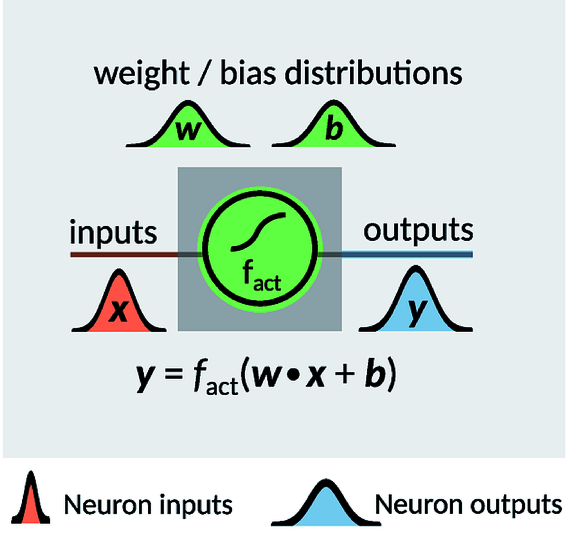
\includegraphics[width=.55\textwidth]{../Images/BNN-neuron.png}
	\caption{Example BNN Neuron \cite{hase2019machine}}
	\label{fig:bnn-neuron}
\end{figure}

\subsubsection{Priors}
\label{subsection:priors}

The Bayesian paradigm requires a prior on the parameters of a neural network to facilitate training. However, making choice of a prior on all the parameters of a network, following anything other than a simple concept, is difficult, especially given the limited understanding of how priors at one layer affects the next in general. For the purposes of this work, only one prior-selection scheme will be considered, since considering many methods would require introducing many further new concepts. 

A choice of prior that is both commonly used and intuitive is an independent normal distribution on each weight. In particular, a $\mathcal{N}(0, \sigma^2)$ distribution with zero mean and some standard deviation $\sigma$ for each particular weight typically works. This can be thought of as a reasonable choice of vague prior. Since further interpretation of how these priors influence the model becomes even more complicated for other priors, selecting a more informative prior would be tricky. For an example of this complexity, Vladimirova et al. contend that for a network with these priors whose activation functions satisfying a certain "extended envelope property", the priors on the $k^{th}$ hidden layer become sub-Weibull-distributed with parameter $k/2$ conditional on the data passing through the network. Such interpretation is valuable, but beyond the scope of this paper.

However, it turns out there is suggestive parallel between a prior in a Bayesian neural network and \textit{regularization} in a typical neural network. \textit{Regularization} is an additional term in the loss that penalizes large weights. Intuitively, this helps resist overfitting by preventing a single neuron from overly influencing the model, since such a neuron may be overemphasizing a fluke of the training set rather than a general pattern. The regularization term typically takes the form $\alpha ||w||_p$  where $||\cdot||_p$ is some choice of metric on $R^n$, typically $p=1$ (Manhattan/taxicab distance) or $p=2$ (Euclidean distance), and $\alpha$ is the regularization hyperparameter that controls how strongly large weights are penalized. In other words, $\alpha$ is the \textit{regularization rate}. 

As in Jospin et al., consider network parameters $\theta$ with a loss function $L$ assumed to be the negative log likelihood loss, where $D_y$ represents the true labels for the training data $D_x$. Suppose the network does not use regularization. Maximum likelihood estimation aims to find the choice of $\theta$ which minimizes the loss on the given data:
$$
\hat{\theta} = \arg \min_{\theta} \left\{ L_{D_x, D_y} (\theta) \right\}.
$$
From the Bayesian perspective, since the negative log likelihood loss is used, this means that
$$
\hat{\theta} = \arg \min_{\theta} \left\{- \log P(D_y|D_x, \theta) \right\} = \arg \max_{\theta} \left\{ P(D_y|D_x, \theta) \right\}.
$$
This formula indicates to find the choice of $\theta$ that maximizes the probability of the true labels $D_y$ for the data given the observed $D_x$ values for parameters $\theta$. Now, suppose a prior $p(\theta)$ is introduced:
$$
\hat{\theta} = \arg \max_{\theta} P(D_y|D_x, \theta) p(\theta).
$$
When converted back to the frequentist paradigm under log-likelihood loss, the multiplicative factor for the prior becomes an additive regularization term:
$$
\hat{\theta} = \arg \min_{\theta} L_{D_x, D_y} (\theta) + reg(\theta), \quad reg(\theta) = -\log(p(\theta)).
$$
Jospin et al. state that normal prior selected above is "equivalent to a weighted $\ell_2$ regularization (with weights $1/\sigma$) when training a point estimate network." In this sense, the Bayesian model which utilizes priors specified in advance helps prevent overfitting simply by including priors in the first place. 

% TODO: Add discussion of how distributions are imposed
%\subsection{Distributions}

%In order to impose distributions on the parameters of a Bayesian neural network, there must be a clearly defined procedure for producting a posterior from the prior and the data. 

%Gradient descent is used to minimize (the approximation of) the KL-divergence...


\subsection{Bayesian Convolutional Neural Networks}

As discussed previously, Bayesian neural networks work with most functional models that work for typical neural networks. Convolutional neural networks are no exception - by simply replacing typical CNNs with Bayesian counterparts containing Bayesian neurons and the appropriate operations, a Bayesian convolutional neural network (BCNN) is created. 

\section{Simulation}

We use an implementation of BCNNs from \href{https://github.com/kumar-shridhar/PyTorch-BayesianCNN}{Github} based on work from \cite{shridhar2019comprehensive} \cite{shridhar2018uncertainty}. It allowed for direct substitution of Bayesian layers for deterministic neural network layers such that the same training procedure could be applied to both types of networks. The normal priors previously discussed are built into these custom layers in the package. 

\subsection{CIFAR-10}

	\begin{figure}[H]
		\centering
	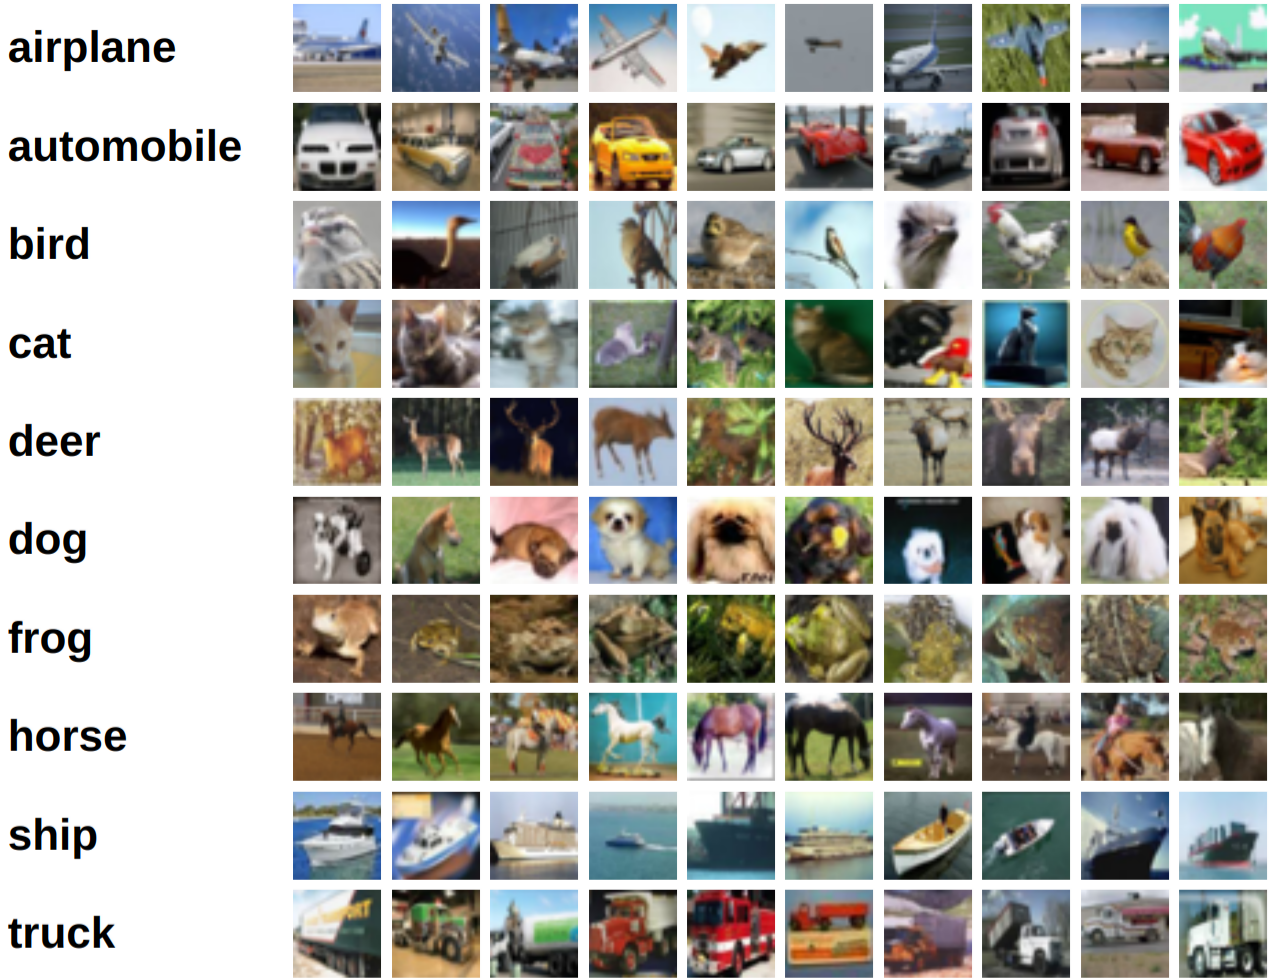
\includegraphics[width=.75\textwidth]{../Images/cifar-10.png}
	\caption{Example CIFAR-10 images \cite{cifar10}}
\end{figure}

The CIFAR-10 (Canadian Institute For Advanced Research 10) dataset is a machine learning benchmarking set. It contains $60,000$ $32 \times 32$ RGB pictures of airplanes, cars, birds, cats, deer, dogs, frogs, horses, ships, and trucks \cite{cifar10}. The ten classes within the dataset are mutually exclusive, meaning there is no image containing multiple of the objects mentioned above. The number of images is split evenly between each class, with $6,000$ images per each type of object. It is a very popular data set (in fact the most common) to use in machine learning and training neural networks, due to the extensive size, as well as the decent number of categories. The purpose of the images within the dataset being of a lower resolution is to allow researchers to see more quickly (and with less computation effort) how well an algorithm works on classification with the dataset. Convolutional neural networks are often seen to be the ``best" at classifying CIFAR-10.

\subsection{Hyperparameters}

The hyperparameters of a neural network, such as epochs, learning rate, regularization rate, are set before training to control the process and ensure the network achieves the best possible performance for its architecture. Epochs and learning rate were defined in Subsection \ref{subsection:neural-network-training} while the regularization rate and its connection to Bayesian network priors was introduced in \ref{subsection:priors}. The choice of optimizer is not relevant to and beyond the scope of this work - Adamw as selected here simply provides a marginal performance improvement. 

We choose to keep the number of layers and levels in the model the same to keep the models roughly equal, but tuned the hyperparameters separately. We did not adjust the priors on the BCNN, as those were set by the BCNN layer code from \cite{shridhar2018uncertainty}. We found the following hyperparemeters created the best model:

\begin{figure}[H]
	\begin{center}
	\begin{tabular}{|c||p{3cm}|p{3cm}|} % Adjust p{width} as needed
	\hline
	\textbf{Hyperparameter} & \textbf{CNN} & \textbf{BCNN} \\ [0.5ex] 
	\hline\hline
	Epochs & 100 & 100\\
	\hline
	Learning Rate & 0.001  & 0.003  \\
	\hline
	Regularization Rate& 0.001 & 0.001 \\
	\hline
	Optimizer & Adamw  & Adamw  \\
	\hline
\end{tabular}
\end{center}
\end{figure}



\subsection{Results}

\begin{figure}[H]
	\centering
	\begin{tabular}{|c||p{3cm}|p{3cm}|} % Adjust p{width} as needed
		\hline
		\textbf{Metric} & \textbf{CNN} & \textbf{BCNN} \\ [0.5ex] 
		\hline\hline
		Train Accuracy & 84.96\% & 81.27\%\\
		\hline
		Validation Accuracy & 61.76\%  & 59.21\%  \\
		\hline
		Time to Train & 16 min 11 sec  & 22 min 11 sec  \\
		\hline
	\end{tabular}
\end{figure}

The results we achieved with training were about the same between the BCNN and the CNN. However, the bayesian model took longer to train.

\begin{figure}[H]
	\centering
	\begin{subfigure}{.5\textwidth}
		\centering
		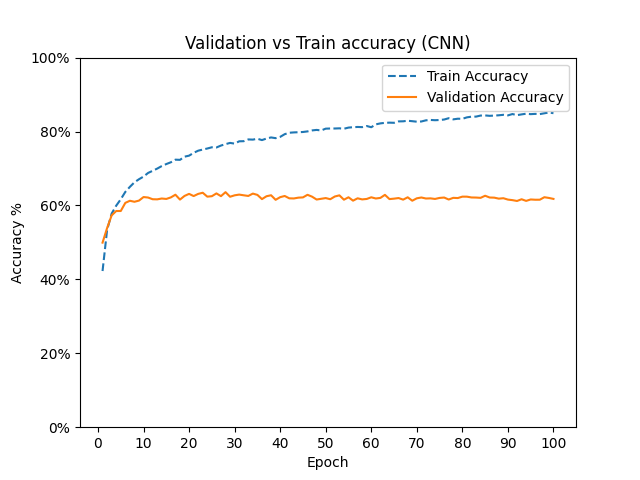
\includegraphics[width=\linewidth]{../Images/CNN_val_acc_over_time}
		\caption{CNN}
	\end{subfigure}% //  
	\begin{subfigure}{.5\textwidth}
		\centering
		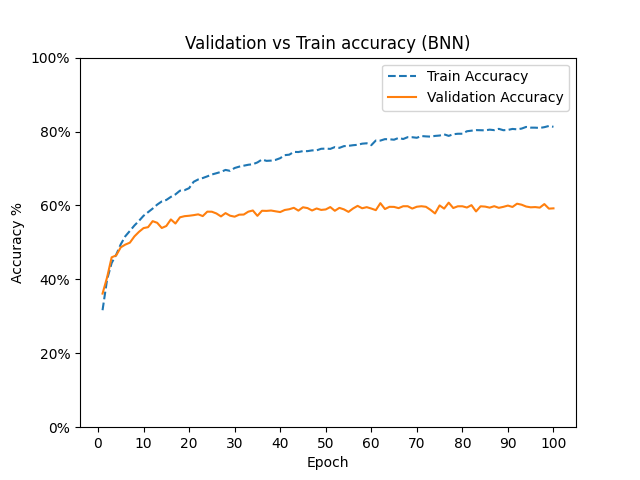
\includegraphics[width=\linewidth]{../Images/BNN_val_acc_over_time}
		\caption{BCNN}
	\end{subfigure}
	\caption{Train vs validation accuracy over time}
	\label{fig:train-v-val}
\end{figure}

Based on the divergent lines in figure \ref{fig:train-v-val}, the model needs tuning. Specifically, the regularization rate needs to be raised. One interesting thing that appears in the figures, is that the BCNN took longer to diverge from the train accuracy compared to CNN.

\begin{figure}[H]
	\centering
	\begin{subfigure}{\textwidth}
		\centering
		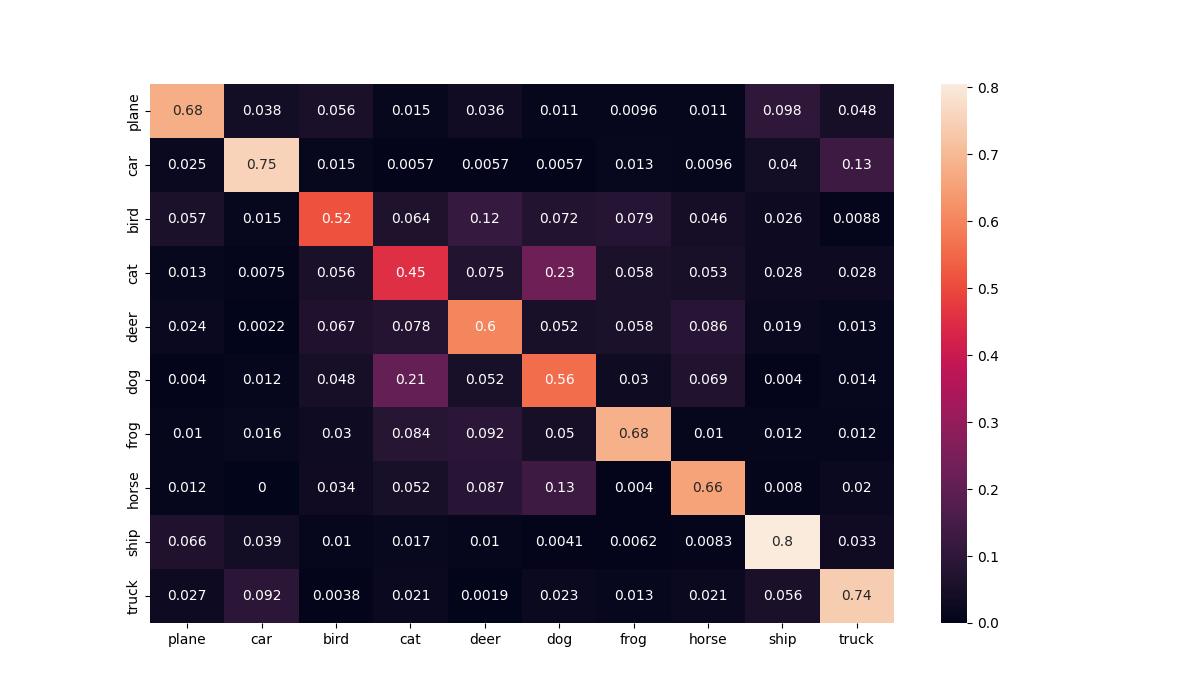
\includegraphics[width=.9\linewidth]{../Images/CNN_confusion_matrix}
		\caption{CNN}
	\end{subfigure} \\% //  
	\begin{subfigure}{\textwidth}
		\centering
		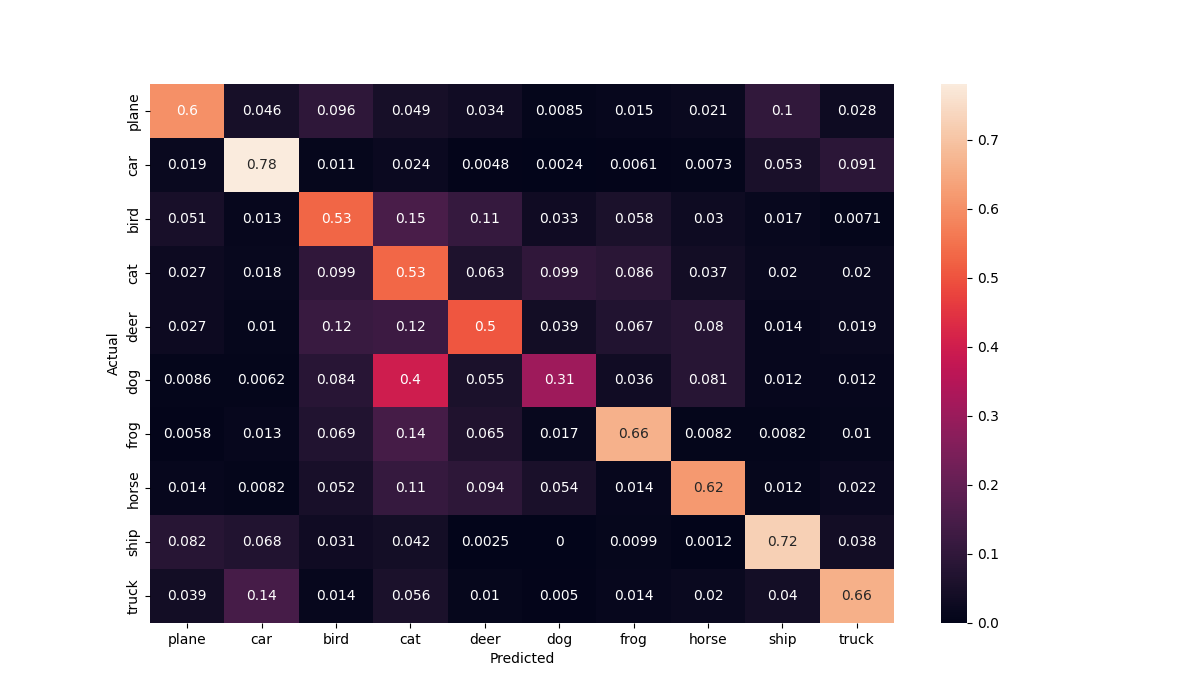
\includegraphics[width=.9\linewidth]{../Images/BNN_confusion_matrix}
		\caption{BCNN}
	\end{subfigure}
	\caption{Confusion matrices}
	\label{fig:confusion}
\end{figure}

Based on the confusion matrix from two models in \ref{fig:confusion}, the two models confuse similar sets of classes. Both models struggle to differentiate animals, but the BCNN has poorer accuracy on the classes that are easily confused. 

\newpage

\printbibliography


\end{document}